%-----------------------------------------------------------------------------------------
% Autor dieser Vorlage:
% Stefan Macke (http://fachinformatiker-anwendungsentwicklung.net)
% Permalink zur Vorlage: http://fiae.link/LaTeXVorlageFIAE
%
% Sämtliche verwendeten Abbildungen, Tabellen und Listings stammen von Dirk Grashorn.
%
% Lizenz: Creative Commons 4.0 Namensnennung - Weitergabe unter gleichen Bedingungen
% -----------------------------------------------------------------------------------------

\documentclass[
	ngerman,
	toc=listof, % Abbildungsverzeichnis sowie Tabellenverzeichnis in das Inhaltsverzeichnis aufnehmen
	toc=bibliography, % Literaturverzeichnis in das Inhaltsverzeichnis aufnehmen
	footnotes=multiple, % Trennen von direkt aufeinander folgenden Fußnoten
	parskip=half, % vertikalen Abstand zwischen Absätzen verwenden anstatt horizontale Einrückung von Folgeabsätzen
	numbers=noendperiod % Den letzten Punkt nach einer Nummerierung entfernen (nach DIN 5008)
]{scrartcl}
\pdfminorversion=5 % erlaubt das Einfügen von pdf-Dateien bis Version 1.7, ohne eine Fehlermeldung zu werfen (keine Garantie für fehlerfreies Einbetten!)
\usepackage[utf8]{inputenc} % muss als erstes eingebunden werden, da Meta/Packages ggfs. Sonderzeichen enthalten

% !TEX root = Projektdokumentation.tex

% Hinweis: der Titel muss zum Inhalt des Projekts passen und den zentralen Inhalt des Projekts deutlich herausstellen
\newcommand{\titel}{Entwicklung von NatInfo}
\newcommand{\untertitel}{Webbasiertes Tool zur Unterstützung der Entwickler}
\newcommand{\kompletterTitel}{\titel{} -- \untertitel}

\newcommand{\autorName}{Stefan Macke}
\newcommand{\autorAnschrift}{Meine Straße 1}
\newcommand{\autorOrt}{49377 Vechta}

\newcommand{\betriebLogo}{LogoBetrieb.pdf}
\newcommand{\betriebName}{\textsc{Alte Oldenburger} Krankenversicherung AG}
\newcommand{\betriebAnschrift}{Alte-Oldenburger-Platz 1}
\newcommand{\betriebOrt}{49377 Vechta}

\newcommand{\ausbildungsberuf}{Fachinformatiker für Anwendungsentwicklung}
\newcommand{\betreff}{Dokumentation zur betrieblichen Projektarbeit}
\newcommand{\pruefungstermin}{Sommer 2015}
\newcommand{\abgabeOrt}{Vechta}
\newcommand{\abgabeTermin}{23.04.2015}
 % Metadaten zu diesem Dokument (Autor usw.)
% !TEX root = ../Projektdokumentation.tex

% Anpassung an Landessprache ---------------------------------------------------
\usepackage{babel}

% Umlaute ----------------------------------------------------------------------
%   Umlaute/Sonderzeichen wie äüöß direkt im Quelltext verwenden (CodePage).
%   Erlaubt automatische Trennung von Worten mit Umlauten.
% ------------------------------------------------------------------------------
\usepackage[T1]{fontenc}
\usepackage{textcomp} % Euro-Zeichen etc.

% Schrift ----------------------------------------------------------------------
\usepackage{lmodern} % bessere Fonts
\usepackage{relsize} % Schriftgröße relativ festlegen

% Tabellen ---------------------------------------------------------------------
\PassOptionsToPackage{table}{xcolor}
\usepackage{tabularx}
% für lange Tabellen
\usepackage{longtable}
\usepackage{array}
\usepackage{ragged2e}
\usepackage{lscape}
\newcolumntype{w}[1]{>{\raggedleft\hspace{0pt}}p{#1}} % Spaltendefinition rechtsbündig mit definierter Breite

% Grafiken ---------------------------------------------------------------------
\usepackage[dvips,final]{graphicx} % Einbinden von JPG-Grafiken ermöglichen
\usepackage{graphics} % keepaspectratio
\usepackage{floatflt} % zum Umfließen von Bildern
\graphicspath{{Bilder/}} % hier liegen die Bilder des Dokuments

% Sonstiges --------------------------------------------------------------------
\usepackage[titles]{tocloft} % Inhaltsverzeichnis DIN 5008 gerecht einrücken
\usepackage{amsmath,amsfonts} % Befehle aus AMSTeX für mathematische Symbole
\usepackage{enumitem} % anpassbare Enumerates/Itemizes
\usepackage{xspace} % sorgt dafür, dass Leerzeichen hinter parameterlosen Makros nicht als Makroendezeichen interpretiert werden

\usepackage{makeidx} % für Index-Ausgabe mit \printindex
\usepackage[printonlyused]{acronym} % es werden nur benutzte Definitionen aufgelistet

% Einfache Definition der Zeilenabstände und Seitenränder etc.
\usepackage{setspace}
\usepackage{geometry}

% Symbolverzeichnis
\usepackage[intoc]{nomencl}
\let\abbrev\nomenclature
\renewcommand{\nomname}{Abkürzungsverzeichnis}
\setlength{\nomlabelwidth}{.25\hsize}
\renewcommand{\nomlabel}[1]{#1 \dotfill}
\setlength{\nomitemsep}{-\parsep}

\usepackage{varioref} % Elegantere Verweise. „auf der nächsten Seite“
\usepackage{url} % URL verlinken, lange URLs umbrechen etc.

\usepackage{chngcntr} % fortlaufendes Durchnummerieren der Fußnoten
% \usepackage[perpage]{footmisc} % Alternative: Nummerierung der Fußnoten auf jeder Seite neu

\usepackage{ifthen} % bei der Definition eigener Befehle benötigt
\usepackage{todonotes} % definiert u.a. die Befehle \todo und \listoftodos
\usepackage[square]{natbib} % wichtig für korrekte Zitierweise

% PDF-Optionen -----------------------------------------------------------------
\usepackage{pdfpages}
\pdfminorversion=5 % erlaubt das Einfügen von pdf-Dateien bis Version 1.7, ohne eine Fehlermeldung zu werfen (keine Garantie für fehlerfreies Einbetten!)
\usepackage[
    bookmarks,
    bookmarksnumbered,
    bookmarksopen=true,
    bookmarksopenlevel=1,
    colorlinks=true,
% diese Farbdefinitionen zeichnen Links im PDF farblich aus
    anchorcolor=AOBlau,% Ankertext
    citecolor=AOBlau, % Verweise auf Literaturverzeichniseinträge im Text
    filecolor=AOBlau, % Verknüpfungen, die lokale Dateien öffnen
    menucolor=AOBlau, % Acrobat-Menüpunkte
    urlcolor=AOBlau,
% diese Farbdefinitionen sollten für den Druck verwendet werden (alles schwarz)
    %linkcolor=black, % einfache interne Verknüpfungen
    %anchorcolor=black, % Ankertext
    %citecolor=black, % Verweise auf Literaturverzeichniseinträge im Text
    %filecolor=black, % Verknüpfungen, die lokale Dateien öffnen
    %menucolor=black, % Acrobat-Menüpunkte
    %urlcolor=black,
%
    %backref, % Quellen werden zurück auf ihre Zitate verlinkt
    pdftex,
    plainpages=false, % zur korrekten Erstellung der Bookmarks
    pdfpagelabels=true, % zur korrekten Erstellung der Bookmarks
    hypertexnames=false, % zur korrekten Erstellung der Bookmarks
    linkcolor=black,
    linktoc=all,
]{hyperref}
% Befehle, die Umlaute ausgeben, führen zu Fehlern, wenn sie hyperref als Optionen übergeben werden
\hypersetup{
    pdftitle={\titel -- \untertitel},
    pdfauthor={\autorName},
    pdfcreator={\autorName},
    pdfsubject={\titel -- \untertitel},
    pdfkeywords={\titel -- \untertitel},
}


% zum Einbinden von Programmcode -----------------------------------------------
\usepackage{listings}
\usepackage{xcolor}
\definecolor{hellgelb}{rgb}{1,1,0.9}
\definecolor{colKeys}{rgb}{0,0,1}
\definecolor{colIdentifier}{rgb}{0,0,0}
\definecolor{colComments}{rgb}{0,0.5,0}
\definecolor{colString}{rgb}{1,0,0}
\lstset{
    float=hbp,
	basicstyle=\footnotesize,
    identifierstyle=\color{colIdentifier},
    keywordstyle=\color{colKeys},
    stringstyle=\color{colString},
    commentstyle=\color{colComments},
    backgroundcolor=\color{hellgelb},
    columns=flexible,
    tabsize=2,
    frame=single,
    extendedchars=true,
    showspaces=false,
    showstringspaces=false,
    numbers=left,
    numberstyle=\tiny,
    breaklines=true,
    breakautoindent=true,
	captionpos=b,
}
\lstdefinelanguage{cs}{
	sensitive=false,
	morecomment=[l]{//},
	morecomment=[s]{/*}{*/},
	morestring=[b]",
	morekeywords={
		abstract,event,new,struct,as,explicit,null,switch
		base,extern,object,this,bool,false,operator,throw,
		break,finally,out,true,byte,fixed,override,try,
		case,float,params,typeof,catch,for,private,uint,
		char,foreach,protected,ulong,checked,goto,public,unchecked,
		class,if,readonly,unsafe,const,implicit,ref,ushort,
		continue,in,return,using,decimal,int,sbyte,virtual,
		default,interface,sealed,volatile,delegate,internal,short,void,
		do,is,sizeof,while,double,lock,stackalloc,
		else,long,static,enum,namespace,string},
}
\lstdefinelanguage{natural}{
	sensitive=false,
	morecomment=[l]{/*},
	morestring=[b]",
	morestring=[b]',
	alsodigit={-,*},
	morekeywords={
		DEFINE,DATA,LOCAL,END-DEFINE,WRITE,CALLNAT,PARAMETER,USING,
		IF,NOT,END-IF,ON,*ERROR-NR,ERROR,END-ERROR,ESCAPE,ROUTINE,
		PERFORM,SUBROUTINE,END-SUBROUTINE,CONST,END-FOR,END,FOR,RESIZE,
		ARRAY,TO,BY,VALUE,RESET,COMPRESS,INTO,EQ},
}
\lstdefinelanguage{php}{
	sensitive=false,
	morecomment=[l]{/*},
	morestring=[b]",
	morestring=[b]',
	alsodigit={-,*},
	morekeywords={
		abstract,and,array,as,break,case,catch,cfunction,class,clone,const,
		continue,declare,default,do,else,elseif,enddeclare,endfor,endforeach,
		endif,endswitch,endwhile,extends,final,for,foreach,function,global,
		goto,if,implements,interface,instanceof,namespace,new,old_function,or,
		private,protected,public,static,switch,throw,try,use,var,while,xor
		die,echo,empty,exit,eval,include,include_once,isset,list,require,
		require_once,return,print,unset},
}
 % verwendete Packages
% !TEX root = ../Projektdokumentation.tex

% Seitenränder -----------------------------------------------------------------
\setlength{\topskip}{\ht\strutbox} % behebt Warnung von geometry
\geometry{a4paper,left=20mm,right=20mm,top=25mm,bottom=35mm}

\usepackage[
	automark, % Kapitelangaben in Kopfzeile automatisch erstellen
	headsepline, % Trennlinie unter Kopfzeile
	ilines % Trennlinie linksbündig ausrichten
]{scrlayer-scrpage}

% Kopf- und Fußzeilen ----------------------------------------------------------
\pagestyle{scrheadings}
% chapterpagestyle gibt es nicht in scrartcl
%\renewcommand{\chapterpagestyle}{scrheadings}
\clearscrheadfoot

% Kopfzeile
\renewcommand{\headfont}{\normalfont} % Schriftform der Kopfzeile
\ihead{\large{\textsc{\titel}}\\ \small{\untertitel} \\[2ex] \textit{\headmark}}
\chead{}
\ohead{\includegraphics[scale=0.2]{\betriebLogo}}
\setlength{\headheight}{15mm} % Höhe der Kopfzeile
%\setheadwidth[0pt]{textwithmarginpar} % Kopfzeile über den Text hinaus verbreitern (falls Logo den Text überdeckt)

% Fußzeile
\ifoot{\autorName}
\cfoot{}
\ofoot{\pagemark}

% Überschriften nach DIN 5008 in einer Fluchtlinie
% ------------------------------------------------------------------------------

% Abstand zwischen Nummerierung und Überschrift definieren
% > Schön wäre hier die dynamische Berechnung des Abstandes in Abhängigkeit
% > der Verschachtelungstiefe des Inhaltsverzeichnisses
\newcommand{\headingSpace}{1.5cm}

% Abschnittsüberschriften im selben Stil wie beim Inhaltsverzeichnis einrücken
\renewcommand*{\othersectionlevelsformat}[3]{
  \makebox[\headingSpace][l]{#3\autodot}
}

% Für die Einrückung wird das Paket tocloft benötigt
%\cftsetindents{chapter}{0.0cm}{\headingSpace}
\cftsetindents{section}{0.0cm}{\headingSpace}
\cftsetindents{subsection}{0.0cm}{\headingSpace}
\cftsetindents{subsubsection}{0.0cm}{\headingSpace}
\cftsetindents{figure}{0.0cm}{\headingSpace}
\cftsetindents{table}{0.0cm}{\headingSpace}


% Allgemeines
% ------------------------------------------------------------------------------

\onehalfspacing % Zeilenabstand 1,5 Zeilen
\frenchspacing % erzeugt ein wenig mehr Platz hinter einem Punkt

% Schusterjungen und Hurenkinder vermeiden
\clubpenalty = 10000
\widowpenalty = 10000
\displaywidowpenalty = 10000

% Quellcode-Ausgabe formatieren
\lstset{numbers=left, numberstyle=\tiny, numbersep=5pt, breaklines=true}
\lstset{emph={square}, emphstyle=\color{red}, emph={[2]root,base}, emphstyle={[2]\color{blue}}}

\counterwithout{footnote}{section} % Fußnoten fortlaufend durchnummerieren
\setcounter{tocdepth}{3} % im Inhaltsverzeichnis werden die Kapitel bis zum Level der subsubsection übernommen
\setcounter{secnumdepth}{3} % Kapitel bis zum Level der subsubsection werden nummeriert

% Aufzählungen anpassen
\renewcommand{\labelenumi}{\arabic{enumi}.}
\renewcommand{\labelenumii}{\arabic{enumi}.\arabic{enumii}.}
\renewcommand{\labelenumiii}{\arabic{enumi}.\arabic{enumii}.\arabic{enumiii}}

% Tabellenfärbung:
\definecolor{heading}{rgb}{0.89,0.72,0.75}
\definecolor{odd}{rgb}{0.9,0.9,0.9}
 % Definitionen zum Aussehen der Seiten
% !TEX root = ../Projektdokumentation.tex

% Abkürzungen, ggfs. mit korrektem Leerraum
\newcommand{\bs}{$\backslash$\xspace}
\newcommand{\bspw}{bspw.\xspace}
\newcommand{\bzw}{bzw.\xspace}
\newcommand{\ca}{ca.\xspace}
\newcommand{\dahe}{\mbox{d.\,h.}\xspace}
\newcommand{\etc}{etc.\xspace}
\newcommand{\eur}[1]{\mbox{#1\,\texteuro}\xspace}
\newcommand{\evtl}{evtl.\xspace}
\newcommand{\ggfs}{ggfs.\xspace}
\newcommand{\Ggfs}{Ggfs.\xspace}
\newcommand{\gqq}[1]{\glqq{}#1\grqq{}}
\newcommand{\inkl}{inkl.\xspace}
\newcommand{\insb}{insb.\xspace}
\newcommand{\ua}{\mbox{u.\,a.}\xspace}
\newcommand{\usw}{usw.\xspace}
\newcommand{\Vgl}{Vgl.\xspace}
\newcommand{\zB}{\mbox{z.\,B.}\xspace}

% Befehle für häufig anfallende Aufgaben
\newcommand{\Abbildung}[1]{\autoref{fig:#1}}
\newcommand{\Anhang}[1]{\appendixname{}~\ref{#1}: \nameref{#1} \vpageref{#1}}
\newcommand{\includegraphicsKeepAspectRatio}[2]{\includegraphics[width=#2\textwidth,height=#2\textheight,keepaspectratio]{#1}}
\newcommand{\Zitat}[2][\empty]{\ifthenelse{\equal{#1}{\empty}}{\citep{#2}}{\citep[#1]{#2}}}
\newcommand{\Autor}[1]{\textsc{#1}} % zum Ausgeben von Autoren
\newcommand{\itemd}[2]{\item{\textbf{#1}}\\{#2}} % erzeugt ein Listenelement mit fetter Überschrift

% fügt Tabellen aus einer TEX-Datei ein
\newcommand{\tabelle}[3] % Parameter: caption, label, file
{\begin{table}[htbp]
\centering
\singlespacing
\input{Tabellen/#3}
\caption{#1}
\label{#2}
\end{table}}

\newcommand{\tabelleAnhang}[1] % Parameter: file
{\begin{center}
\singlespacing
\input{Tabellen/#1}
\end{center}}

% einfaches Wechseln der Schrift, z.B.: \changefont{cmss}{sbc}{n}
\newcommand{\changefont}[3]{\fontfamily{#1} \fontseries{#2} \fontshape{#3} \selectfont}

% Verwendung analog zu \includegraphics
\newlength{\myx} % Variable zum Speichern der Bildbreite
\newlength{\myy} % Variable zum Speichern der Bildhöhe
\newcommand\includegraphicstotab[2][\relax]{%
% Abspeichern der Bildabmessungen
\settowidth{\myx}{\includegraphics[{#1}]{#2}}%
\settoheight{\myy}{\includegraphics[{#1}]{#2}}%
% das eigentliche Einfügen
\parbox[c][1.1\myy][c]{\myx}{%
\includegraphics[{#1}]{#2}}%
}

\definecolor{AOBlau}{rgb}{0, 0.28, 0.56}

% verschiedene Befehle um Wörter semantisch auszuzeichnen ----------------------
\newcommand{\Index}[2][\empty]{\ifthenelse{\equal{#1}{\empty}}{\index{#2}#2}{\index{#1}#2}}
\newcommand{\Fachbegriff}[2][\empty]{\ifthenelse{\equal{#1}{\empty}}{\textit{\Index{#2}}}{\textit{\Index[#1]{#2}}}}
\newcommand{\NeuerBegriff}[2][\empty]{\ifthenelse{\equal{#1}{\empty}}{\textbf{\Index{#2}}}{\textbf{\Index[#1]{#2}}}}

\newcommand{\Ausgabe}[1]{\texttt{#1}}
\newcommand{\Eingabe}[1]{\texttt{#1}}
\newcommand{\Code}[1]{\texttt{#1}}
\newcommand{\Datei}[1]{\texttt{#1}}

\newcommand{\Assembly}[1]{\textsf{#1}}
\newcommand{\Klasse}[1]{\textsf{#1}}
\newcommand{\Methode}[1]{\textsf{#1}}
\newcommand{\Attribut}[1]{\textsf{#1}}

\newcommand{\Datentyp}[1]{\textsf{#1}}
\newcommand{\XMLElement}[1]{\textsf{#1}}
\newcommand{\Webservice}[1]{\textsf{#1}}

\newcommand{\Refactoring}[1]{\Fachbegriff{#1}}
\newcommand{\CodeSmell}[1]{\Fachbegriff{#1}}
\newcommand{\Metrik}[1]{\Fachbegriff{#1}}
\newcommand{\DesignPattern}[1]{\Fachbegriff{#1}}
 % eigene allgemeine Befehle, die z.B. die Arbeit mit LaTeX erleichtern
% Abkürzungen
\newcommand{\Versis}{\textsc{Versis}\xspace}
\newcommand{\NI}{NatInfo\xspace}
\newcommand{\AO}{\textsc{Alte Oldenburger} Krankenversicherung\xspace}
 % eigene projektspezifische Befehle, z.B. Abkürzungen usw.

\begin{document}

\phantomsection
\thispagestyle{empty}
\pdfbookmark[1]{Eidesstattliche Erklärung}{ihkdeckblatt}
\includegraphicsKeepAspectRatio{DeckblattIHK}{1}
\cleardoublepage

\phantomsection
\thispagestyle{plain}
\pdfbookmark[1]{Deckblatt}{deckblatt}
% !TEX root = Projektdokumentation.tex
\begin{titlepage}

\begin{center}

\includegraphics[scale=0.25]{LogoIHK.pdf}\\[1ex]
\Large{Abschlussprüfung \pruefungstermin}\\[3ex]

\Large{\ausbildungsberuf}\\
\LARGE{\betreff}\\[4ex]

\huge{\textbf{\titel}}\\[1.5ex]
\Large{\textbf{\untertitel}}\\[4ex]

\normalsize
Abgabetermin: \abgabeOrt, den \abgabeTermin\\[3em]
\textbf{Prüfungsbewerber:}\\
\autorName\\
\autorAnschrift\\
\autorOrt\\[5ex]

\includegraphics[scale=0.4]{\betriebLogo}\\[2ex]
\textbf{Ausbildungsbetrieb:}\\
\betriebName\\
\betriebAnschrift\\
\betriebOrt\\[5em]
\end{center}

\end{titlepage}
\cleardoublepage

% Preface --------------------------------------------------------------------
\phantomsection
\pagenumbering{Roman}
\pdfbookmark[1]{Inhaltsverzeichnis}{inhalt}
\tableofcontents

\cleardoublepage

\phantomsection
\listoffigures
\cleardoublepage

\phantomsection
\listoftables
\cleardoublepage

\phantomsection
\lstlistoflistings
\cleardoublepage

\newcommand{\abkvz}{Abkürzungsverzeichnis}
\renewcommand{\nomname}{\abkvz}
\section*{\abkvz}
\markboth{\abkvz}{\abkvz}
\addcontentsline{toc}{section}{\abkvz}
% !TEX root = Projektdokumentation.tex

% Es werden nur die Abkürzungen aufgelistet, die mit \ac definiert und auch benutzt wurden. 
%
% \acro{VERSIS}{Versicherungsinformationssystem\acroextra{ (Bestandsführungssystem)}}
% Ergibt in der Liste: VERSIS Versicherungsinformationssystem (Bestandsführungssystem)
% Im Text aber: \ac{VERSIS} -> Versicherungsinformationssystem (VERSIS)

% Hinweis: allgemein bekannte Abkürzungen wie z.B. bzw. u.a. müssen nicht ins Abkürzungsverzeichnis aufgenommen werden
% Hinweis: allgemein bekannte IT-Begriffe wie Datenbank oder Programmiersprache müssen nicht erläutert werden,
%          aber ggfs. Fachbegriffe aus der Domäne des Prüflings (z.B. Versicherung)

% Die Option (in den eckigen Klammern) enthält das längste Label oder
% einen Platzhalter der die Breite der linken Spalte bestimmt.
\begin{acronym}[WWWWW]
	\acro{AO}{\textsc{Alte Oldenburger} Krankenversicherung AG}
	\acro{API}{Application Programming Interface}
	\acro{CSS}{Cascading Style Sheets}
	\acro{CSV}{Comma Separated Value}
	\acro{EPK}{Ereignisgesteuerte Prozesskette}
	\acro{ERM}{En\-ti\-ty-Re\-la\-tion\-ship-Mo\-dell}
	\acro{HTML}{Hypertext Markup Language}\acused{HTML}
	\acro{IDE}{Integrated Development Environment}
	\acro{MVC}[MVC]{Model View Controller}
	\acro{NatInfo}[\textsc{NatInfo}]{Natural Information System}
	\acro{Natural}[\textsc{Natural}]{Programmiersprache der Software AG}\acused{Natural}
	\acro{ORM}{Object-Relational Mapping}
	\acro{PHP}{Hypertext Preprocessor}
	\acro{SDK}{Software Development Kit}
	\acro{SQL}{Structured Query Language}
	\acro{SVN}{Subversion}
	\acro{UML}{Unified Modeling Language}
	\acro{XML}{Extensible Markup Language}
\end{acronym}

\clearpage

% Inhalt ---------------------------------------------------------------------
\pagenumbering{arabic}
% !TEX root = Projektdokumentation.tex
% !TEX root = ../Projektdokumentation.tex
\section{Einleitung}
\label{sec:Einleitung}


\subsection{Projektumfeld} 
\label{sec:Projektumfeld}

\subsubsection{Ausbildungsbetrieb}

Die \textbf{LUPCOM media GmbH} ist eine Internetagentur mit ihrem Hauptsitz in Rostock, die sich darauf spezialisiert hat, Webseiten und Webanwendungen für eine vielfältige Kundschaft zu entwerfen und zu entwickeln. Ihr Fokus liegt darauf, maßgeschneiderte Lösungen zu bieten, die den individuellen Anforderungen und Größenordnungen ihrer Kunden entsprechen. Dabei deckt sie ein breites Spektrum von Projekten ab, von kleinen Unternehmenswebseiten bis hin zu komplexen Webanwendungen. Für die Umsetzung dieser Projekte werden Technologien wie Contao, Symfony, JavaScript sowie Docker verwendet.

\subsubsection{Kunde}

Der Auftraggeber dieses Projekts ist die \textbf{MS "Ostseebad Rerik"}, ein Ausflugsschiff, das entlang der „verbotenen“ Halbinsel Wustrow fährt. Das Schiff bietet mehrmals täglich in der Hauptsaison Rundfahrten auf dem Salzhaff an, die etwa zwei Stunden dauern und unter kundiger Führung des Kapitäns stattfinden. Zusätzlich bietet die MS "Ostseebad Rerik" gastronomische Versorgung sowie Charterfahrten für Jubiläen, Betriebsfeiern und Vereinsausflüge an.


\subsection{Projektziel} 
\label{sec:Projektziel}

Ziel dieses Projekts ist die Entwicklung eines zuverlässigen und effizienten QR-Code-basierten Einlösungsprogramms. Dieses Programm soll den Einlösungsprozess digitalisieren und automatisieren. Konkret umfasst das Projektziel die folgenden Punkte:

\begin{itemize}
    \item \textbf{Generierung einzigartiger QR-Codes für spezifische Bestellungen:} Für jede Bestellung soll ein individueller QR-Code generiert werden, der durch einen Mitarbeiter eingescannt und entwertet werden kann.
    \item \textbf{Sichere und effiziente Einlösung durch Scannen der QR-Codes:} Die QR-Codes sollen von den Mitarbeitern gescannt werden können, um die Echtheit und Gültigkeit der Tickets oder Gutscheine sofort zu überprüfen.
    \item \textbf{Intuitive Benutzeroberfläche für die Überprüfung der Bestellinformationen und die Entwertung der Tickets/Gutscheine:} Das System soll eine benutzerfreundliche Oberfläche bieten, die es den Mitarbeitern ermöglicht, die Bestellinformationen schnell und einfach einzusehen und die Tickets oder Gutscheine nach der Einlösung zu entwerten.
	\item \textbf{Einfache Installation mittels composer:} Die Anwendung muss mit dem Paketmanager composer kompatibel sein, um eine einfache Installation zu gewährleisten.
\end{itemize}

Durch die Erfüllung dieser Ziele wird das Projekt erfolgreich abgeschlossen.

\subsection{Projektbegründung} 
\label{sec:Projektbegruendung}

Die Durchführung dieses Projekts soll mehrere bestehende Probleme im aktuellen Einlösungsprozess beheben und sowohl die Effizienz als auch die Zufriedenheit der Mitarbeiter steigern.

\subsubsection{Aktuelles Problem}
Der aktuelle Prozess zur Überprüfung und Einlösung von online erworbenen Tickets und Gutscheinen basiert auf manuellen Methoden. Diese manuelle Verifizierung ist zeitaufwendig und fehleranfällig, was zu einer ineffizienten Nutzung der Arbeitszeit führt und die Kundenzufriedenheit negativ beeinflusst.

\subsubsection{Vorteile des QR-Code-basierten Systems}
Die Entwicklung eines QR-Code-basierten Einlösungsprogramms bietet zahlreiche Vorteile:

\begin{itemize}
    \item \textbf{Reduktion von Fehlern:} Durch die Automatisierung des Verifizierungsprozesses werden menschliche Fehler minimiert, was die Zuverlässigkeit der Ticket- und Gutscheinüberprüfung erhöht.
    \item \textbf{Zeitersparnis:} Mitarbeiter können QR-Codes schnell scannen und sofortige Rückmeldungen über die Gültigkeit der Tickets erhalten, was den gesamten Prozess beschleunigt.
    \item \textbf{Erhöhte Sicherheit:} Das System gewährleistet eine sichere Einlösung von Tickets und Gutscheinen, wodurch Betrugsversuche reduziert werden.
    \item \textbf{Verbesserte Kundenzufriedenheit:} Ein effizienter und schneller Einlösungsprozess steigert das Kundenerlebnis und das Vertrauen in die digitalen Dienstleistungen.
\end{itemize}

\subsubsection{Vorteile für die Mitarbeiter}
Die Einführung eines QR-Code-basierten Einlösungsprogramms soll die Mitarbeiter vor Ort entlasten:

\begin{itemize}
    \item \textbf{Erleichterung der Arbeitsabläufe:} Die Automatisierung reduziert den manuellen Aufwand und die Komplexität der Aufgaben, was die Arbeitslast der Mitarbeiter verringert.
    \item \textbf{Steigerung der Produktivität:} Mitarbeiter können ihre Zeit effizienter nutzen und sich auf andere wichtige Aufgaben konzentrieren.
    \item \textbf{Verbesserte Arbeitsqualität:} Durch die Minimierung von Fehlern und die Vereinfachung der Prozesse wird die Qualität der Arbeit verbessert, was zu höherer Arbeitszufriedenheit führt.
\end{itemize}

Insgesamt soll die Implementierung eines QR-Code-basierten Einlösungsprogramms zu einer Verbesserung der Effizienz und Qualität der Arbeitsabläufe sowie zu einer gesteigerten Zufriedenheit der Mitarbeiter und Kunden führen.

\subsection{Projektschnittstellen} 
\label{sec:Projektschnittstellen}

Die Anwendung soll verschiedene Schnittstellen bereitstellen, um eine nahtlose Integration und effiziente Nutzung zu gewährleisten. Im Folgenden werden die geplanten Schnittstellen beschrieben.

\subsubsection{Technische Schnittstellen}

\begin{itemize}
    \item \textbf{Interaktion mit Shop-Systemen:} Die Anwendung soll sich nahtlos in die bestehenden Shop-Systeme integrieren. Hierbei soll für jede Bestellung ein einzigartiger QR-Code generiert werden, der in den Bestelldaten gespeichert und den Kunden zur Verfügung gestellt wird.
    \item \textbf{API-Schnittstellen:} Die Anwendung soll mehrere API-Endpunkte bereitstellen, um die Interaktion mit externen Systemen und die Verarbeitung der QR-Codes zu ermöglichen. Dies umfasst Endpunkte für die Validierung und Entwertung der QR-Codes sowie die Bereitstellung der entsprechenden Bestelldetails.
\end{itemize}

\subsubsection{Präsentation der Ergebnisse}

\begin{itemize}
    \item \textbf{Benutzeroberfläche:} Die Ergebnisse der QR-Code-Verifizierung und Einlösung sollen über eine benutzerfreundliche Oberfläche präsentiert werden.
    \item \textbf{Darstellung für Mitarbeiter:} Die Bestellinformationen sollen den Mitarbeitern in einem klaren und strukturierten Format präsentiert werden, um eine schnelle und effiziente Überprüfung und Entwertung der Tickets zu ermöglichen. Dies umfasst die Anzeige der Bestelldetails wie Bestellnummer, Datum und Status sowie den Entwertungsstatus.
\end{itemize}


\subsection{Projektabgrenzung} 
\label{sec:Projektabgrenzung}
\begin{itemize}
	\item Was ist explizit nicht Teil des Projekts (\insb bei Teilprojekten)?
\end{itemize}

% !TEX root = ../Projektdokumentation.tex
\section{Projektplanung} 
\label{sec:Projektplanung}


\subsection{Projektphasen}
\label{sec:Projektphasen}

Für die Umsetzung des Projekts standen insgesamt 80 Stunden zur Verfügung, die vor Beginn auf verschiedene Phasen der Softwareentwicklung verteilt wurden. Die Projektarbeit erstreckte sich über zwei 4-Tage-Wochen, ergänzt durch zwei zusätzliche Arbeitstage, um Feiertage auszugleichen. Die Durchführung erfolgte vom 25.04.2024 bis 26.04.2024, sowie vom 29.04.2024 bis 03.05.2024 und vom 20.05.2024 bis 24.05.2024, jeweils mit einer täglichen Arbeitszeit von 8 Stunden.

Eine Übersicht der groben Zeitplanung und der Hauptphasen findet sich in Tabelle 1: Grobe Zeitplanung. Diese Hauptphasen sind weiter in detaillierte Unterabschnitte gegliedert, um eine präzise Planung zu gewährleisten. Eine detaillierte Darstellung der Phasen ist im Anhang A.1: Detaillierte Zeitplanung auf Seite i zu finden.

\paragraph{Tabelle~\ref{tab:Zeitplanung}} zeigt die grobe Zeitplanung.
\tabelle{Zeitplanung}{tab:Zeitplanung}{ZeitplanungKurz}\\
Eine detailliertere Zeitplanung findet sich im \Anhang{app:Zeitplanung}.


\subsection{Abweichungen vom Projektantrag}
\label{sec:AbweichungenProjektantrag}

Zunächst war in der Zeitplanung des Projektantrags die Erstellung eines Abnahmeprotokolls vorgesehen. Dieses Protokoll wurde jedoch nicht erstellt. Stattdessen erfolgte die Übergabe der Projektergebnisse direkt an die zuständige Abteilung, die die Abnahme informell durch ein einfaches Abnicken bestätigte.

Des Weiteren waren im Projektantrag Unit-Tests eingeplant, um die Qualität des Codes sicherzustellen. Aufgrund von Zeitmangel konnten diese Tests jedoch nicht durchgeführt werden. Stattdessen wurden manuelle Tests durchgeführt, bei denen die Arbeitsabläufe durch manuelles Durchklicken überprüft wurden.

Eine weitere Abweichung betraf die Erstellung der Entwürfe. Im Projektantrag war vorgesehen, dass diese aufgrund ihrer erwarteten geringen Anzahl vom Autor erstellt werden. Allerdings stellte sich während des Projekts heraus, dass die Anzahl der erforderlichen Benutzeroberflächen umfangreicher war als angenommen. Daher wurde beschlossen, die Entwürfe an die Design-Abteilung zu übergeben. Lediglich die Ticketansicht und die Popups wurden vom Autor entworfen.

Auch die Benutzerdokumentation fiel kleiner aus als ursprünglich geplant. Dies lag daran, dass die Abnahme durch die Fachabteilung mehr Zeit in Anspruch nahm als vorgesehen, was die Zeit für die Erstellung der Dokumentation verkürzte.

\subsection{Ressourcenplanung}
\label{sec:Ressourcenplanung}

\begin{itemize}
	\item Detaillierte Planung der benötigten Ressourcen (Hard-/Software, Räumlichkeiten \usw).
	\item \Ggfs sind auch personelle Ressourcen einzuplanen (\zB unterstützende Mitarbeiter).
	\item Hinweis: Häufig werden hier Ressourcen vergessen, die als selbstverständlich angesehen werden (\zB PC, Büro). 
\end{itemize}


\subsection{Entwicklungsprozess}
\label{sec:Entwicklungsprozess}
\begin{itemize}
	\item Welcher Entwicklungsprozess wird bei der Bearbeitung des Projekts verfolgt (\zB Wasserfall, agiler Prozess)?
\end{itemize}

% !TEX root = ../Projektdokumentation.tex
\section{Analysephase} 
\label{sec:Analysephase}


\subsection{Ist-Analyse} 
\label{sec:IstAnalyse}

Der aktuelle Prozess zur Überprüfung der Echtheit und Gültigkeit von Tickets und Gutscheinen basiert auf manuellen Methoden. Dies führt zu einer hohen Fehleranfälligkeit und ist zudem äußerst ineffizient. Die Mitarbeiter sind gezwungen, viel Zeit in die Überprüfung der Tickets zu investieren, was ihre Effizienz erheblich mindert.

Die Wünsche der Mitarbeiter beinhalten eine schnellere und zuverlässigere Methode zur Überprüfung von Tickets und Gutscheinen. Es besteht ein klarer Bedarf an einer automatisierten Lösung, die menschliche Fehler minimiert und den Verifizierungsprozess beschleunigt. Die Mitarbeiter wollen ihre Zeit effektiver nutzen und sich auf wichtigere Aufgaben konzentrieren können.

Das Ziel des Projekts ist es, ein QR-Code-basiertes Einlösungsprogramm zu erstellen, das diese Probleme adressiert. Durch die Implementierung eines Systems, das QR-Codes generiert und scannt, wird die Echtheit und Gültigkeit der Tickets schnell und sicher überprüft. Dies verbessert nicht nur die Effizienz der Arbeitsabläufe, sondern erhöht auch die Zuverlässigkeit und Sicherheit des gesamten Prozesses. Insgesamt führt die Automatisierung zu einer gesteigerten Zufriedenheit sowohl der Mitarbeiter als auch der Kunden.

\subsubsection{\gqq{Make or Buy}-Entscheidung}
\label{sec:MakeOrBuyEntscheidung}

Bei der Entscheidung, ob eine bestehende Lösung verwendet oder eine neue entwickelt werden sollte, wurde sorgfältig geprüft, ob es bereits ein fertiges Produkt gibt, das alle Anforderungen des Projekts abdeckt. Dabei stellte sich heraus, dass es keine existierende Lösung gab, die den spezifischen Anforderungen entsprach.

Ein wichtiges Kriterium war die Kompatibilität mit dem bereits genutzten Framework Contao und dem Onlineshop-Plugin Isotope. Die Suche nach einer fertigen Lösung, die als Bundle über Composer installiert werden kann und nahtlos mit Contao und Isotope zusammenarbeitet, war erfolglos. Die vorhandenen Produkte auf dem Markt deckten entweder nicht alle funktionalen Anforderungen ab oder waren nicht vollständig kompatibel mit der bestehenden Architektur.

Aufgrund dieser speziellen Anforderungen und der fehlenden passenden Lösungen auf dem Markt wurde entschieden, das Projekt intern umzusetzen. Dies ermöglichte eine maßgeschneiderte Entwicklung, die exakt auf die Bedürfnisse des Unternehmens und der Mitarbeiter zugeschnitten ist. Durch die interne Entwicklung konnte sichergestellt werden, dass alle Anforderungen vollständig erfüllt und gleichzeitig die bestehende Architektur optimal genutzt wird.

\subsubsection{Projektkosten}
\label{sec:Projektkosten}

\paragraph{Rechnung}
Die Kosten für die Durchführung des Projekts setzen sich sowohl aus Personal-, als auch aus Ressourcenkosten zusammen. Für Azubis gilt ein pauschaler Stundensatz von 50€. Für fest angestellte Mitarbeiter gilt ein Stundensatz von 89€.

Die Durchführungszeit des Projekts beträgt 80 Stunden. Die Nutzung von Ressourcen wie Räumlichkeiten, Arbeitsplatzrechner etc.\ sind bereits in diesem Stundensatz enthalten.

Eine Aufstellung der Kosten befindet sich in Tabelle~\ref{tab:Kostenaufstellung} und sie betragen insgesamt \eur{6002,50}.
\tabelle{Kostenaufstellung}{tab:Kostenaufstellung}{Kostenaufstellung.tex}


\subsubsection{Wirtschaftlichkeit / Amortisationsdauer}
\label{sec:Amortisationsdauer}

Da das System intern entwickelt wurde, entfallen Ausgaben für externe Softwarelizenzen, Updates und Wartungsverträge. Dies reduziert die langfristigen Betriebskosten und führt zu direkten Kosteneinsparungen.

Durch die interne Entwicklung des Systems vermeiden wir zudem die Kosten für die Anpassung und Integration externer Lösungen. Die Anwendung ist exakt auf die Bedürfnisse unserer Kunden und die von uns unterstützten Plattformen abgestimmt, was zusätzliche Anpassungsarbeiten überflüssig macht.

Ein weiterer signifikanter Vorteil ist die Zeitersparnis bei der Implementierung und dem Support. Dank der engen Integration mit dem bestehenden Contao-Framework und dem Isotope-Shop-Plugin können Entwickler das System schnell und mit wenig Komplikationen einrichten. Die reduzierte Implementierungszeit bedeutet, dass wir mehr Projekte in kürzerer Zeit abschließen können, was zu einer höheren Umsatzrate führt.

Zusätzlich ermöglicht uns das QR-Code-System, unsere Marktposition zu stärken und als technologischer Vorreiter wahrgenommen zu werden. Die Fähigkeit, moderne Lösungen anzubieten, verbessert unsere Wettbewerbsfähigkeit und hilft dabei, neue Kunden zu gewinnen und bestehende Kundenbeziehungen zu vertiefen.

Durch den Verkauf des Programms an mehrere Kunden können wir außerdem von wiederkehrenden Einnahmen profitieren. Wartungsverträge, Schulungen und zusätzliche Supportdienste bieten kontinuierliche Einkommensströme.

\paragraph{Rechnung}
Die Projektkosten für die Entwicklung des Programms betrugen insgesamt 6002,50€. Das Projekt wurde erfolgreich für 7200€ verkauft. Das ergibt einen direkten Umsatz nach Abnahme des Projekts, von \eur{1197.50}.

\subsection{Anwendungsfälle}
\label{sec:Anwendungsfaelle}

Der erste Anwendungsfall betrifft die Generierung eines QR-Codes für eine Bestellung. Sobald ein Kunde im Onlineshop eine Bestellung abschließt, wird automatisch ein einzigartiger QR-Code generiert. Dieser QR-Code enthält alle relevanten Bestelldaten und wird in der Datenbank gespeichert. Anschließend wird der QR-Code per E-Mail an den Kunden versendet. Dies ermöglicht eine einfache und sichere Verifizierung der Bestellung.

Ein weiterer zentraler Anwendungsfall ist die Verifizierung und Einlösung des QR-Codes durch einen Mitarbeiter. Der Kunde präsentiert den QR-Code, den er per E-Mail erhalten hat. Der Mitarbeiter scannt den QR-Code, und das System überprüft dessen Gültigkeit. Ist der QR-Code gültig, werden dem Mitarbeiter alle relevanten Informationen zur Bestellung angezeigt. Der Mitarbeiter kann dann entscheiden, ob er den QR-Code tatsächlich einlösen möchte. Nach der Bestätigung wird der QR-Code im System als eingelöst markiert und kann nicht erneut verwendet werden. Dies stellt sicher, dass jeder QR-Code nur einmal genutzt werden kann und verhindert Betrugsversuche.

Zusätzlich gibt es die Möglichkeit einer manuelle Suche nach den Tickets. Sollte es einmal nicht möglich sein, den QR-Code zu scannen, kann der Mitarbeiter nach einem Ticket suchen. Das Programm zeigt dann die Gültigkeit des Tickets an und gibt die entsprechenden Bestellinformationen aus, um die Einlösung zu ermöglichen.

\paragraph{Use Case-Diagramm}
Ein Use Case-Diagramm befindet sich im \Anhang{app:UseCase}.

\subsection{Qualitätsanforderungen}
\label{sec:Qualitaetsanforderungen}

Ein zentraler Qualitätsaspekt ist die Fehlerfreiheit der Anwendung. Es sollten möglichst wenig Fehler in der Benutzung auftreten. Falls dennoch Fehler auftreten, muss klar und verständlich kommuniziert werden, was falsch gelaufen ist. Die Fehlermeldungen sollten in einer Form präsentiert werden, die dem Benutzer nützliche Informationen liefert, um das Problem zu beheben oder den Support zu kontaktieren. Kritische Fehler, die das gesamte Programm lahmlegen, sind unbedingt zu vermeiden.

Die Zuverlässigkeit des Systems ist ein weiterer wichtiger Faktor. Benutzer müssen sich darauf verlassen können, dass ein als gültig angezeigtes Ticket tatsächlich gültig ist. Das System sollte sich so gut wie möglich vor gefälschten oder manipulierten Tickets schützen. Ein Fehler in der Verifizierung der Tickets kann zu erheblichen finanziellen Verlusten für den Kunden führen. Daher muss das System stets korrekte und verlässliche Ergebnisse liefern.

Die Usability der Anwendung spielt ebenfalls eine große Rolle. Die Benutzeroberfläche sollte intuitiv und benutzerfreundlich gestaltet sein, sodass auch unerfahrene Benutzer problemlos mit dem System arbeiten können.

Die Integrationsfähigkeit in die bestehende Umgebung spielt auch eine entscheidende Rolle. Das Programm muss sich nahtlos in die vorhandene Infrastruktur integrieren lassen und die vorgegebene Struktur von Symfony Bundles einhalten. Dies gewährleistet eine reibungslose Integration in bestehende Systeme und erleichtert die Wartung und Erweiterung der Anwendung.

Das Programm muss außerdem sicherstellen, dass nur Mitarbeiter mit einem hinterlegten Login Zugang zu dem Einlösetool haben. Diese Maßnahme verhindert, dass Tickets versehentlich entwertet werden oder sensible Bestellinformationen von unbefugten Personen eingesehen werden können.

\subsection{Lastenheft/Fachkonzept}
\label{sec:Lastenheft}
Alle spezifischen Anforderungen sowie die allgemeinen, technischen und qualitativen Ziele, die im Rahmen dieses Projekts festgelegt wurden, sind detailliert im Lastenheft beschrieben. Für eine umfassende Übersicht und weitere Details wird auf das \Anhang{app:Lastenheft} verwiesen.

% !TEX root = ../Projektdokumentation.tex
\section{Entwurfsphase} 
\label{sec:Entwurfsphase}

\subsection{Zielplattform}
\label{sec:Zielplattform}

\textbf{Programmiersprache:} Die Anwendung wird in PHP unter Verwendung des Symfony-Frameworks entwickelt. Symfony bietet eine robuste und flexible Grundlage für Webanwendungen und unterstützt die Erstellung von sicheren und skalierbaren Lösungen. Die Wahl von PHP und Symfony ermöglicht eine effiziente Entwicklung und Wartung der Anwendung.

\textbf{Datenbank:} Als Datenbank wird MySQL eingesetzt. MySQL ist eine weit verbreitete, leistungsstarke und zuverlässige relationale Datenbank, die gut mit Symfony und PHP integriert werden kann. Sie bietet die notwendige Leistung und Stabilität, um die Bestelldaten und QR-Codes sicher zu speichern und schnell abzurufen.

\textbf{Client/Server-Architektur:} Die Anwendung wird als Webanwendung mit einer Client/Server-Architektur implementiert. Dies ermöglicht eine zentrale Verwaltung und Aktualisierung der Anwendung auf dem Server, während die Benutzer über ihre Webbrowser auf die Anwendung zugreifen. Die Verwendung einer Webanwendung stellt sicher, dass keine zusätzliche Software auf den Endgeräten der Benutzer installiert werden muss.

\textbf{Hardware:} Die Zielplattform umfasst Smartphones, da diese über integrierte Kameras verfügen, die für das Scannen der QR-Codes erforderlich sind. Die Anwendung soll auf allen Smartphones mit Webbrowsern und einer Internetverbindung zugänglich sein. Dies stellt sicher, dass alle Mitarbeiter unabhängig vom verwendeten Gerät auf die Anwendung zugreifen können.

Die Entscheidung für PHP, Symfony und MySQL fiel, weil diese Technologien in unserem Betrieb gängig sind und von unseren Entwicklern routiniert verwendet werden. Dadurch kann effizient und schnell gearbeitet werden. Zudem ermöglicht diese Kombination die Erstellung von Composer-Bundles, die sich nahtlos in andere Symfony-Projekte integrieren lassen.

Besonders wichtig ist dies, weil das Kundenprojekt, in dem das Bundle eingebunden werden soll, Contao verwendet, welches auf Symfony basiert. Diese Auswahl an Technologien erleichtert die Implementierung und gewährleistet eine konsistente Benutzererfahrung.

\subsection{Architekturdesign}
\label{sec:Architekturdesign}

Für das QR-Code-basierte Einlösungsprogramm wurde das Symfony-Framework ausgewählt, das die Grundlage für das verwendete Contao CMS bildet. Diese Entscheidung wurde sowohl aufgrund der spezifischen Anforderungen des Projekts als auch der etablierten Praktiken im Betrieb getroffen. Symfony und Contao bieten eine leistungsfähige Kombination, die auf dem Model-View-Controller (\acs{MVC}) Muster basiert. Dieses Architekturmuster teilt die Anwendung in drei Hauptkomponenten: Modell, Ansicht und Controller.

Das MVC-Modell ermöglicht eine klare Trennung der Geschäftslogik von der Benutzeroberfläche. Diese Struktur erleichtert die Arbeit am Projekt, da die Logik der QR-Code-Generierung und -Verifizierung unabhängig von der Präsentation implementiert werden kann.

Ein zentraler Vorteil von Symfony und Contao liegt in der nativen Unterstützung von Composer, welches die Erstellung von Bundles ermöglicht. Ein Bundle fungiert als eine Art Plugin oder Modul, das bestimmte Funktionen kapselt und wiederverwendbar macht. Im Rahmen dieses Projekts wird das QR-Code-Tool als Bundle entwickelt, wodurch es sich problemlos in andere Contao-Projekte integrieren lässt.

Für die Authentifizierung der Benutzer kann die Mitgliedsverwaltung von Contao genutzt werden. Dies stellt sicher, dass nur autorisierte Benutzer auf das Einlösetool zugreifen können und sensible Bestellinformationen geschützt bleiben.

Die integrierten Sicherheitsmechanismen von Symfony, einschließlich der Benutzer-Authentifizierung und -Autorisierung, stellen sicher, dass die Anwendung vor unbefugtem Zugriff geschützt ist und die Integrität der Bestelldaten gewahrt bleibt.


\subsection{Datenmodell}
\label{sec:Datenmodell}

Ein Entity-Relationship-Modell (ERM) ist im \Anhang{app:Datenbankmodell} zu finden.

\begin{figure}[htb]
\centering
\includegraphicsKeepAspectRatio{ERDiagramm.pdf}{0.6}
\caption{Vereinfachtes ER-Modell}
\label{fig:ER}
\end{figure} 


\subsection{Geschäftslogik}
\label{sec:Geschaeftslogik}

\begin{itemize}
	\item Modellierung und Beschreibung der wichtigsten (!) Bereiche der Geschäftslogik (\zB mit Kom\-po\-nen\-ten-, Klassen-, Sequenz-, Datenflussdiagramm, Programmablaufplan, Struktogramm, \ac{EPK}).
	\item Wie wird die erstellte Anwendung in den Arbeitsfluss des Unternehmens integriert?
\end{itemize}

\paragraph{Beispiel}
Ein Klassendiagramm, welches die Klassen der Anwendung und deren Beziehungen untereinander darstellt kann im \Anhang{app:Klassendiagramm} eingesehen werden.

\Abbildung{Modulimport} zeigt den grundsätzlichen Programmablauf beim Einlesen eines Moduls als \ac{EPK}.
\begin{figure}[htb]
\centering
\includegraphicsKeepAspectRatio{modulimport.pdf}{0.9}
\caption{Prozess des Einlesens eines Moduls}
\label{fig:Modulimport}
\end{figure}


\subsection{Maßnahmen zur Qualitätssicherung}
\label{sec:Qualitaetssicherung}

Die Überprüfung der korrekten Ausführung des Codes erfolgte mithilfe des Debug-Modus von Symfony und auslesen von Log-Dateien. Durch dieses Debugging konnten potenzielle Fehlerquellen identifiziert und behoben werden, bevor sie zu größeren Problemen führten.

Es wurden außerdem Frontend-Tests durchgeführt, um die Funktionalität und Benutzerfreundlichkeit der Anwendung sicherzustellen. Diese Tests beinhalteten die Simulation der typischen Benutzerinteraktionen, wie das Scannen und Verifizieren von QR-Codes, sowie die Überprüfung der Navigations- und Anzeigeelemente. Ziel war es, sicherzustellen, dass alle erforderlichen Features reibungslos funktionieren und die Anwendung intuitiv bedienbar ist.

Die Sicherheitsaspekte der Anwendung wurden ebenfalls getestet. Dies umfasste die Zugangskontrolle, bei der überprüft wurde, dass nur autorisierte Mitarbeiter mit einem hinterlegten Login auf das Einlösetool zugreifen können. Dadurch wurde gewährleistet, dass sensible Bestellinformationen geschützt und Tickets nicht versehentlich entwertet werden.

\subsection{Pflichtenheft/Datenverarbeitungskonzept}
\label{sec:Pflichtenheft}

Für die Implementierungsdetails dieses Projekts wird auf das im Anhang befindliche Pflichtenheft verwiesen. Dieses Dokument wurde im Verlauf des Projekts erarbeitet und dient als umfassende Guideline, die alle notwendigen Schritte und Vorgaben zur erfolgreichen Realisierung der Anwendung enthält. Das Pflichtenheft ist im \Anhang{app:Pflichtenheft} zu finden.
% !TEX root = ../Projektdokumentation.tex
\section{Implementierungsphase} 
\label{sec:Implementierungsphase}

\subsection{Implementierung der Datenstrukturen}
\label{sec:ImplementierungDatenstrukturen}

Contao generiert die Datenbanktabellen automatisch anhand der DCA-Dateien, die im \texttt{dca/} Ordner des jeweiligen Bundles hinterlegt sind. Eine DCA-Datei enthält die Konfiguration für eine Datenbanktabelle, einschließlich der Definition der Felder und deren Eigenschaften. Beim Installations- oder Aktualisierungsprozess liest Contao diese Konfigurationsdateien aus und erstellt oder aktualisiert die entsprechenden Tabellen in der Datenbank.

Die DCA-Datei definiert die Struktur und die Felder der Tabelle, einschließlich der SQL-Typen und anderer relevanter Einstellungen. Contao interpretiert diese Informationen und generiert die erforderlichen SQL-Befehle, um die Datenbanktabellen anzulegen oder zu aktualisieren.

Die Tabelle \texttt{tl\_iso\_order\_hashes} wurde erstellt, um die QR-Codes und deren zugehörige Informationen zu verwalten.

\begin{itemize}
    \item \textbf{id}: Dieses Feld dient als Primärschlüssel und wird automatisch hochgezählt. Es wird als \texttt{int(10) unsigned} definiert, um eine ausreichende Anzahl von Einträgen zu ermöglichen.
    \item \textbf{hash}: Dieses Feld speichert den aus Bestellinformationen generierten Hash-Wert. Es ist als \texttt{varchar(64)} definiert, um den Hash-Wert aufzunehmen, wobei 64 Zeichen ausreichend für einen sicheren Hash-Wert sind.
    \item \textbf{iso\_product\_collection\_id}: Dieses Feld speichert die ID der zugehörigen Produktkollektion aus dem Isotope-Shop. Es wird als \texttt{int(10)} definiert.
    \item \textbf{valid}: Dieses Feld definiert die Gültigkeit des QR-Codes. Es ist als \texttt{int(1)} definiert, wobei der Standardwert \texttt{0} ist. Ein Wert von \texttt{1} bedeutet, dass der QR-Code gültig und noch nicht eingelöst ist.
\end{itemize}

Ein Screenshot der DCA-Datei wird im Anhang bereitgestellt, um eine visuelle Darstellung der Konfiguration zu bieten. Der Screenshot ist hier zu finden: \Anhang{app:ScreenshotDca}.

\subsection{Implementierung der Benutzeroberfläche}
\label{sec:ImplementierungBenutzeroberflaeche}

\begin{itemize}
	\item Beschreibung der Implementierung der Benutzeroberfläche, falls dies separat zur Implementierung der Geschäftslogik erfolgt (\zB bei \acs{HTML}-Oberflächen und Stylesheets).
	\item \Ggfs Beschreibung des Corporate Designs und dessen Umsetzung in der Anwendung.
	\item Screenshots der Anwendung
\end{itemize}

\paragraph{Beispiel}
Screenshots der Anwendung in der Entwicklungsphase mit Dummy-Daten befinden sich im \Anhang{Screenshots}.


\subsection{Implementierung der Geschäftslogik}
\label{sec:ImplementierungGeschaeftslogik}

\begin{itemize}
	\item Beschreibung des Vorgehens bei der Umsetzung/Programmierung der entworfenen Anwendung.
	\item \Ggfs interessante Funktionen/Algorithmen im Detail vorstellen, verwendete Entwurfsmuster zeigen.
	\item Quelltextbeispiele zeigen.
	\item Hinweis: Wie in Kapitel~\ref{sec:Einleitung}: \nameref{sec:Einleitung} zitiert, wird nicht ein lauffähiges Programm bewertet, sondern die Projektdurchführung. Dennoch würde ich immer Quelltextausschnitte zeigen, da sonst Zweifel an der tatsächlichen Leistung des Prüflings aufkommen können.
\end{itemize}

\paragraph{Beispiel}
Die Klasse \texttt{Com\-par\-ed\-Na\-tu\-ral\-Mo\-dule\-In\-for\-ma\-tion} findet sich im \Anhang{app:CNMI}.  

% !TEX root = ../Projektdokumentation.tex
\section{Abnahmephase} 
\label{sec:Abnahmephase}

\begin{itemize}
	\item Welche Tests (\zB Unit-, Integrations-, Systemtests) wurden durchgeführt und welche Ergebnisse haben sie geliefert (\zB Logs von Unit Tests, Testprotokolle der Anwender)?
	\item Wurde die Anwendung offiziell abgenommen?
\end{itemize}

\paragraph{Beispiel}
Ein Auszug eines Unit Tests befindet sich im \Anhang{app:Test}. Dort ist auch der Aufruf des Tests auf der Konsole des Webservers zu sehen.

% !TEX root = ../Projektdokumentation.tex
\section{Einführungsphase}
\label{sec:Einfuehrungsphase}

\begin{itemize}
	\item Welche Schritte waren zum Deployment der Anwendung nötig und wie wurden sie durchgeführt (automatisiert/manuell)?
	\item Wurden \ggfs Altdaten migriert und wenn ja, wie?
	\item Wurden Benutzerschulungen durchgeführt und wenn ja, Wie wurden sie vorbereitet?
\end{itemize}

% !TEX root = ../Projektdokumentation.tex
\section{Dokumentation}
\label{sec:Dokumentation}

\begin{itemize}
	\item Wie wurde die Anwendung für die Benutzer/Administratoren/Entwickler dokumentiert (\zB Benutzerhandbuch, \acs{API}-Dokumentation)?
	\item Hinweis: Je nach Zielgruppe gelten bestimmte Anforderungen für die Dokumentation (\zB keine IT-Fachbegriffe in einer Anwenderdokumentation verwenden, aber auf jeden Fall in einer Dokumentation für den IT-Bereich).
\end{itemize}

Ein Beispiel der dokumentierten PHP-Funktionen befindet sich im \Anhang{app:BenutzerDoku}.

% !TEX root = ../Projektdokumentation.tex
\section{Fazit} 
\label{sec:Fazit}

\subsection{Soll-/Ist-Vergleich}
\label{sec:SollIstVergleich}

\begin{itemize}
	\item Wurde das Projektziel erreicht und wenn nein, warum nicht?
	\item Ist der Auftraggeber mit dem Projektergebnis zufrieden und wenn nein, warum nicht?
	\item Wurde die Projektplanung (Zeit, Kosten, Personal, Sachmittel) eingehalten oder haben sich Abweichungen ergeben und wenn ja, warum?
	\item Hinweis: Die Projektplanung muss nicht strikt eingehalten werden. Vielmehr sind Abweichungen sogar als normal anzusehen. Sie müssen nur vernünftig begründet werden (\zB durch Änderungen an den Anforderungen, unter-/überschätzter Aufwand).
\end{itemize}

\paragraph{Beispiel (verkürzt)}
Wie in Tabelle~\ref{tab:Vergleich} zu erkennen ist, konnte die Zeitplanung bis auf wenige Ausnahmen eingehalten werden.
\tabelle{Soll-/Ist-Vergleich}{tab:Vergleich}{Zeitnachher.tex}


\subsection{Lessons Learned}
\label{sec:LessonsLearned}

\begin{itemize}
	\item Was hat der Prüfling bei der Durchführung des Projekts gelernt (\zB Zeitplanung, Vorteile der eingesetzten Frameworks, Änderungen der Anforderungen)?
\end{itemize}


\subsection{Ausblick}
\label{sec:Ausblick}

\begin{itemize}
	\item Wie wird sich das Projekt in Zukunft weiterentwickeln (\zB geplante Erweiterungen)?
\end{itemize}


% Literatur ------------------------------------------------------------------
\clearpage
\renewcommand{\refname}{Literaturverzeichnis}
\bibliography{Bibliographie}
\bibliographystyle{Allgemein/natdin} % DIN-Stil des Literaturverzeichnisses
% !TEX root = Projektdokumentation.tex
\clearpage
\addsec{Eidesstattliche Erklärung}

% Hinweis: die eidesstattliche Erklärung ist ggfs. an die Richtlinie der IHK anzupassen

Ich, \autorName, versichere hiermit, dass ich meine \textbf{\betreff} mit dem
Thema
\begin{quote}
\textit{\kompletterTitel}
\end{quote}
selbständig verfasst und keine anderen als die angegebenen Quellen und Hilfsmittel benutzt habe,
wobei ich alle wörtlichen und sinngemäßen Zitate als solche gekennzeichnet habe. Die Arbeit
wurde bisher keiner anderen Prüfungsbehörde vorgelegt und auch nicht veröffentlicht.\\[6ex]

\abgabeOrt, den \abgabeTermin


\rule[-0.2cm]{5.5cm}{0.5pt}

\textsc{\autorName}


% Anhang ---------------------------------------------------------------------
\clearpage
\appendix
\pagenumbering{roman}
% !TEX root = Projektdokumentation.tex
\section{Anhang}
\subsection{Detaillierte Zeitplanung}
\label{app:Zeitplanung}

\tabelleAnhang{ZeitplanungKomplett}

\subsection{Übersicht Ressourcenplanung}
\label{app:Ressourcenplanung}

\tabelleAnhang{Ressourcenplanung}

\subsection{Lastenheft (Auszug)}
\label{app:Lastenheft}
Es folgt ein Auszug aus dem Lastenheft mit Fokus auf die Anforderungen:

Die Anwendung muss folgende Anforderungen erfüllen:
\begin{enumerate}[itemsep=0em,partopsep=0em,parsep=0em,topsep=0em]
    \item Generierung und Verwaltung von QR-Codes
    \begin{enumerate}
        \item Die Anwendung muss für jede abgeschlossene Bestellung einen einzigartigen QR-Code generieren.
        \item Es muss ein Eintrag für jedes Ticket in die Datenbank geschrieben werden.
        \item Die QR-Codes müssen per E-Mail an die Kunden versendet werden.
    \end{enumerate}

    \item Einlösung und Verifizierung von QR-Codes
    \begin{enumerate}
        \item Die Anwendung muss das Scannen der QR-Codes ermöglichen.
        \item Die Anwendung muss die Gültigkeit der gescannten QR-Codes überprüfen.
        \item Die Anwendung muss die Bestellinformationen anzeigen, wenn ein QR-Code gescannt wird.
        \item Die Anwendung muss es ermöglichen, die Einlösung der QR-Codes zu bestätigen und diese als eingelöst zu markieren.
        \item Ungültige oder bereits eingelöste QR-Codes dürfen nicht erneut akzeptiert werden.
    \end{enumerate}

    \item Benutzeroberfläche und Usability
    \begin{enumerate}
        \item Die Benutzeroberfläche muss intuitiv und benutzerfreundlich gestaltet sein.
        \item Die Navigation durch die Anwendung muss einfach und klar strukturiert sein.
        \item Fehlermeldungen müssen verständlich und hilfreich sein, um dem Benutzer bei der Problembehebung zu helfen.
    \end{enumerate}

    \item Sicherheit und Zugriffskontrolle
    \begin{enumerate}
        \item Die Anwendung muss vor gefälschten und manipulierten QR-Codes sicher sein.
        \item Es muss sichergestellt werden, dass nur autorisierte Mitarbeiter mit einem hinterlegten Login Zugang zur Anwendung haben.
        \item Die Zugriffskontrolle muss verhindern, dass unbefugte Personen sensible Bestellinformationen einsehen oder Tickets versehentlich entwerten können.
    \end{enumerate}

    \item Integrationsfähigkeit
    \begin{enumerate}
        \item Die Anwendung muss sich nahtlos in die bestehende Systemlandschaft integrieren.
        \item Die Struktur der Anwendung muss den Anforderungen eines Symfony Bundles entsprechen.
    \end{enumerate}

    \item Zuverlässigkeit und Effizienz
    \begin{enumerate}
        \item Die Anwendung muss verlässlich und korrekt arbeiten.
        \item Kritische Fehler, die das gesamte Programm lahmlegen, müssen unbedingt vermieden werden.
    \end{enumerate}
\end{enumerate}


\clearpage

\subsection{Use Case-Diagramm}
\label{app:UseCase}

\begin{figure}[h]
    \centering
    \begin{tikzpicture}
        \usetikzlibrary{shapes,arrows}
        \tikzstyle{actor}=[draw, ellipse, fill=gray!20, minimum height=2em]
        \tikzstyle{usecase}=[draw, ellipse, minimum height=2em, minimum width=3em]

        \node [actor] (employee) {Mitarbeiter};
        \node [usecase, right=of employee, yshift=2cm] (scan) {QR-Code scannen};
        \node [usecase, below of=scan] (check) {Gültigkeit prüfen};
        \node [usecase, below of=check] (display) {Ticketinformationen anzeigen};
        \node [usecase, below of=display] (confirm) {Einlösung bestätigen};
        \node [usecase, below of=confirm] (invalidate) {QR-Code als ungültig markieren};

        \draw [->] (employee) -- (scan);
        \draw [->] (scan) -- (check);
        \draw [->] (check) -- (display);
        \draw [->] (display) -- (confirm);
        \draw [->] (confirm) -- (invalidate);

        \node [below of=employee, yshift=-3cm] (note) {Kunde zeigt QR-Code aus E-Mail vor};

        \draw [dashed, ->] (note) -- (scan);
    \end{tikzpicture}
    \caption{Use-Case-Diagramm: Einlösung des QR-Codes durch einen Mitarbeiter}
    \label{fig:use_case_diagram}
\end{figure}

\subsection{Pflichtenheft (Auszug)}
\label{app:Pflichtenheft}

\subsubsection*{Zielbestimmung}

\begin{enumerate}[itemsep=0em,partopsep=0em,parsep=0em,topsep=0em]
    \item \textbf{Generierung und Verwaltung von QR-Codes}
    \begin{enumerate}
        \item Das Programm wird eine Funktion zur automatischen Generierung eines einzigartigen QR-Codes für jede abgeschlossene Bestellung implementieren.
        \item Die QR-Codes werden mithilfe einer Bibliothek namens \texttt{php-qrcode} erstellt. Diese Bibliothek ermöglicht es eine Zeichenkette in einen QR-Code zu verwandeln.
        \item Jeder generierte QR-Code wird in der Datenbank gespeichert. Dazu wird eine Tabelle \texttt{tl\_iso\_order\_hashes} verwendet, die die QR-Codes zusammen mit der zugehörigen Bestell-ID und weiteren Metadaten speichert.
        \item Die generierten QR-Codes werden automatisch per E-Mail an die Kunden versendet. Dafür wird eine E-Mail-Versandfunktion integriert, die die QR-Codes als Anhang oder Bild in die E-Mail einfügt.
    \end{enumerate}
    
    \item \textbf{Einlösung und Verifizierung von QR-Codes}
    \begin{enumerate}
        \item Das Programm wird eine Scanfunktion bereitstellen, die mithilfe der Bibliothek \texttt{html5-qrcode} die QR-Codes mit der Kamera eines mobilen Endgeräts scannt.
        \item Die Gültigkeit der gescannten QR-Codes wird überprüft, indem der QR-Code mit den in der Datenbank gespeicherten Hashes abgeglichen wird. Es wird sichergestellt, dass der QR-Code gültig und nicht bereits eingelöst ist.
        \item Nach dem Scannen eines QR-Codes zeigt das Programm die relevanten Bestellinformationen an, die aus der Datenbank abgerufen werden. Diese Informationen umfassen die Bestellnummer, den Namen des Kunden und die Details der Bestellung.
        \item Die Einlösung der QR-Codes wird im System markiert, indem der Status des QR-Codes in der Datenbank auf "eingelöst" gesetzt wird. Dies verhindert die erneute Nutzung des gleichen QR-Codes.
        \item Das Programm stellt sicher, dass ungültige oder bereits eingelöste QR-Codes nicht akzeptiert werden, indem es eine entsprechende Fehlermeldung anzeigt.
    \end{enumerate}

    \item \textbf{Benutzeroberfläche und Usability}
    \begin{enumerate}
        \item Die Benutzeroberfläche wird mithilfe von HTML5-Templates und SCSS entwickelt. Diese Templates werden so gestaltet, dass sie intuitiv und benutzerfreundlich sind.
        \item Die Navigation innerhalb des Programms wird klar und logisch strukturiert, sodass Benutzer leicht zwischen den verschiedenen Funktionen wechseln können.
        \item Fehlermeldungen werden klar formuliert und hilfreich gestaltet, um den Benutzern die Lösung von Problemen zu erleichtern. Für das anzeigen dynamischer Fehlermeldungen wird JavaScript verwendet.
    \end{enumerate}

    \item \textbf{Sicherheit und Zugriffskontrolle}
    \begin{enumerate}
        \item Das Programm wird Maßnahmen zum Schutz vor gefälschten und manipulierten QR-Codes integrieren.
        \item Es wird sichergestellt, dass nur autorisierte Mitarbeiter Zugang zum Programm haben. Dies wird durch die Mitgliedsverwaltung in Contao realisiert, die den Zugriff auf bestimmte Funktionen und Daten einschränkt.
        \item Die Zugriffskontrolle verhindert, dass unbefugte Personen sensible Bestellinformationen einsehen oder Tickets versehentlich entwerten können.
    \end{enumerate}

    \item \textbf{Integrationsfähigkeit}
    \begin{enumerate}
        \item Das Programm wird als Symfony Bundle entwickelt, das sich nahtlos in die bestehende Contao-Umgebung integrieren lässt. Dies erleichtert die Installation und Wartung.
        \item Die Struktur des Programms entspricht den Anforderungen eines Symfony Bundles, sodass es problemlos in andere Projekte eingebunden werden kann.
    \end{enumerate}

    \item \textbf{Zuverlässigkeit und Effizienz}
    \begin{enumerate}
        \item Das Programm wird so entwickelt, dass es zuverlässig und korrekt arbeitet. Dies wird durch manuelle Frontend-Tests sichergestellt.
    \end{enumerate}
\end{enumerate}

\subsubsection*{Produkteinsatz}

\begin{enumerate}[itemsep=0em,partopsep=0em,parsep=0em,topsep=0em]
    \item Anwendungsbereiche\\
    Das QR-Code-basierte Einlösungsprogramm dient zur Verwaltung und Verifizierung von Online-Tickets. Es soll eine effiziente und sichere Abwicklung der Ticketverkäufe und deren Einlösung vor Ort ermöglichen.

    \item Zielgruppen\\
    Die Hauptnutzer der Anwendung sind unsere Kunden, die für die Verifizierung und Einlösung der Tickets ihrer Online-Shops verantwortlich sind. Dazu gehören insbesondere Mitarbeiter in der Veranstaltungsbranche, im Einzelhandel sowie im Tourismusbereich.

    \item Betriebsbedingungen\\
    Die Anwendung muss auf Smartphones mit Webbrowser und Internetverbindung lauffähig sein. Das Programm wird als Webanwendung bereitgestellt. Eine ständige Verfügbarkeit der Anwendung ist durch den Betrieb auf einem Webserver sichergestellt. Updates und Wartungen werden zentral durchgeführt, um die kontinuierliche Verfügbarkeit zu gewährleisten.
\end{enumerate}

\subsection{Datenbankmodell}
\label{app:Datenbankmodell}
ER-Modelle kann man auch direkt mit \LaTeX{} zeichnen, siehe \zB \url{http://www.texample.net/tikz/examples/entity-relationship-diagram/}.
\begin{figure}[htb]
\centering
\includegraphicsKeepAspectRatio{database.pdf}{1}
\caption{Datenbankmodell}
\end{figure}
\clearpage
\subsection{Screenshots des Codes}
\label{ScreenhotsCode}

\subsubsection{DCA}
\label{app:ScreenshotDca}
\begin{figure}[htb]
\centering
\includegraphicsKeepAspectRatio{iso_order_hashes.pdf}{1}
\caption{Datenbankdefinition in iso\_order\_hashes.php}
\end{figure}
\clearpage
% \begin{figure}[htb]
% \centering
% \includegraphicsKeepAspectRatio{modulliste.pdf}{1}
% \caption{Liste der Module mit Filtermöglichkeiten}
% \end{figure}
% \clearpage

\subsection{Screenshots der Anwendung}
\label{Screenshots}
\begin{figure}[htb]
\centering
\includegraphicsKeepAspectRatio{tagliste.pdf}{1}
\caption{Anzeige und Filterung der Module nach Tags}
\end{figure}
\clearpage
\begin{figure}[htb]
\centering
\includegraphicsKeepAspectRatio{modulliste.pdf}{1}
\caption{Liste der Module mit Filtermöglichkeiten}
\end{figure}
\clearpage

\subsection{Entwicklerdokumentation}
\label{app:Doc}
\begin{center}
% Dokumentierte PHP-Funktionen
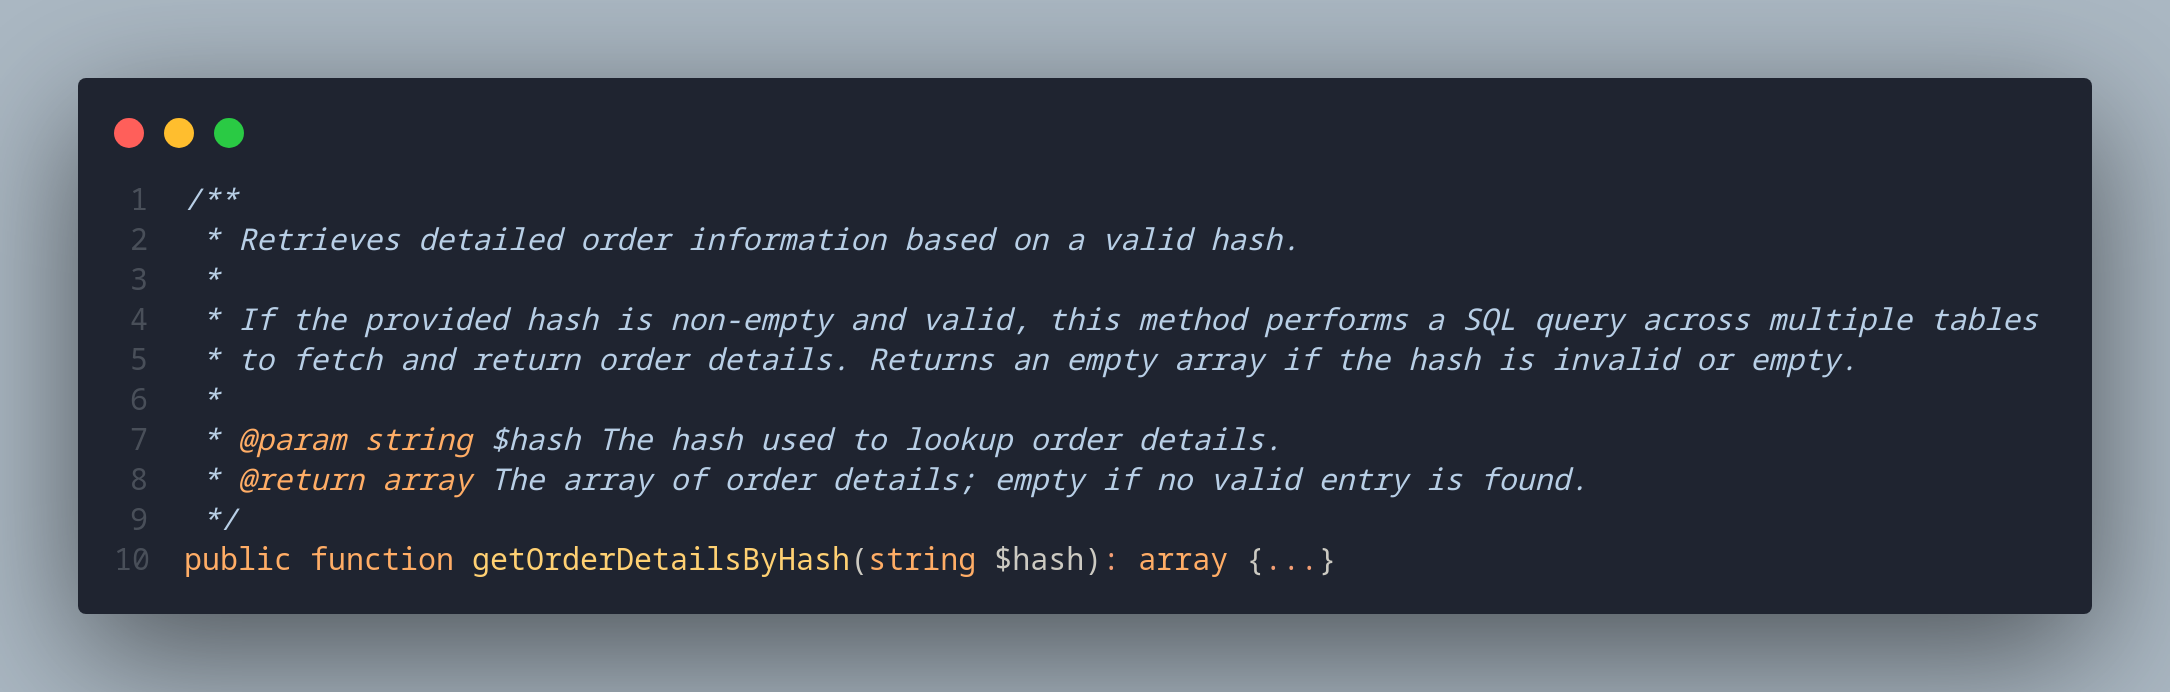
\includegraphics[page=1, width=1\textwidth]{getOrderDetailsByHash.png}
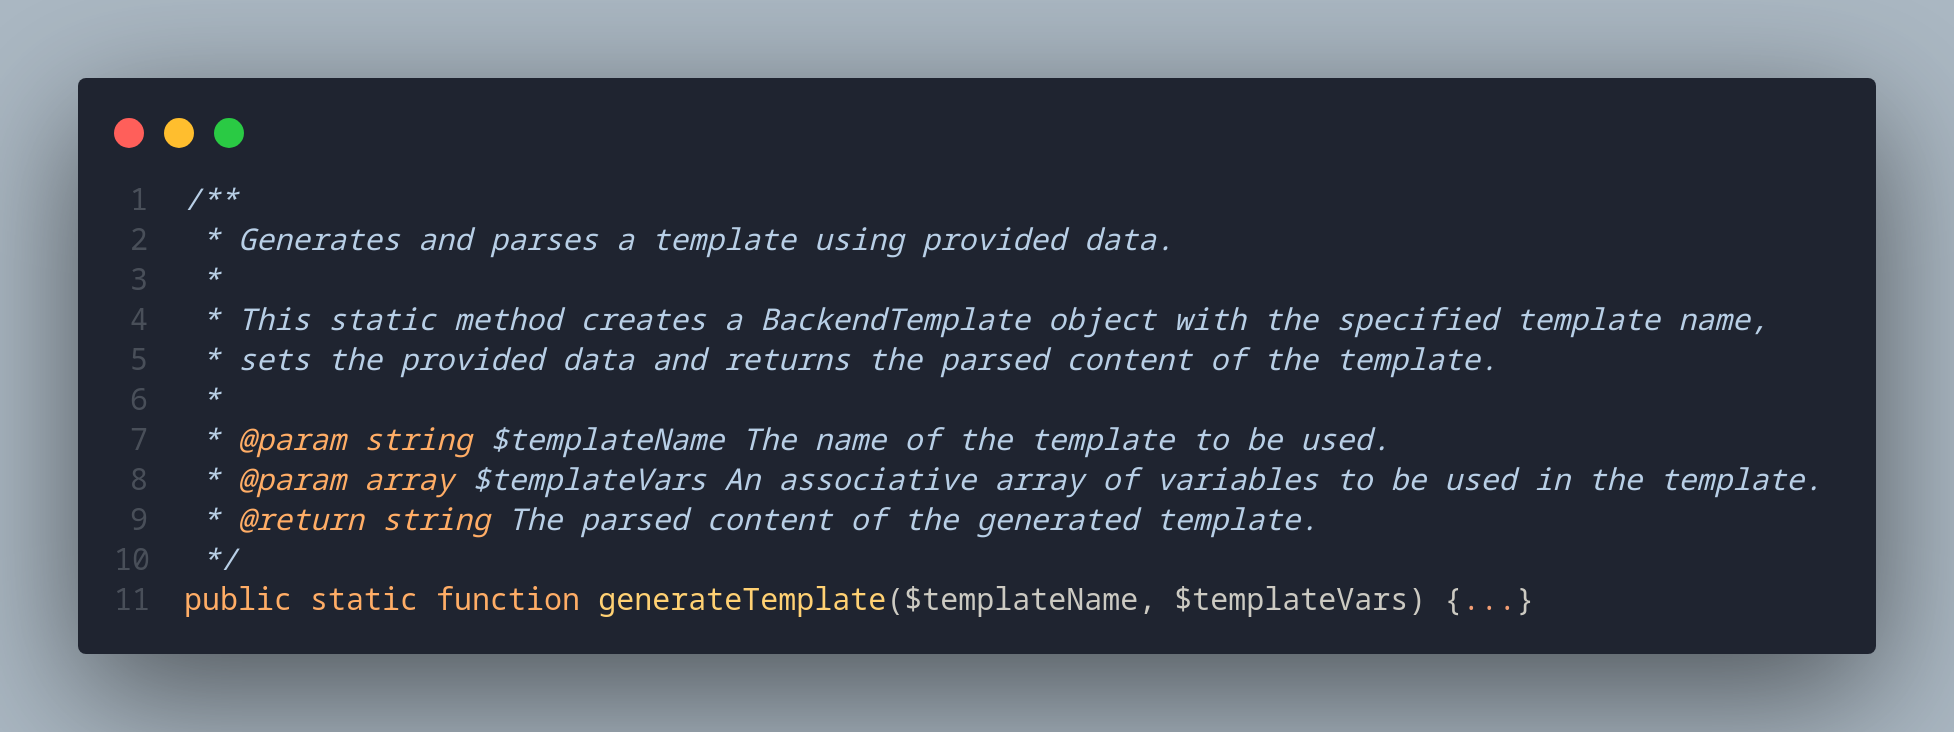
\includegraphics[page=1, width=1\textwidth]{generateTemplateHelper.png}
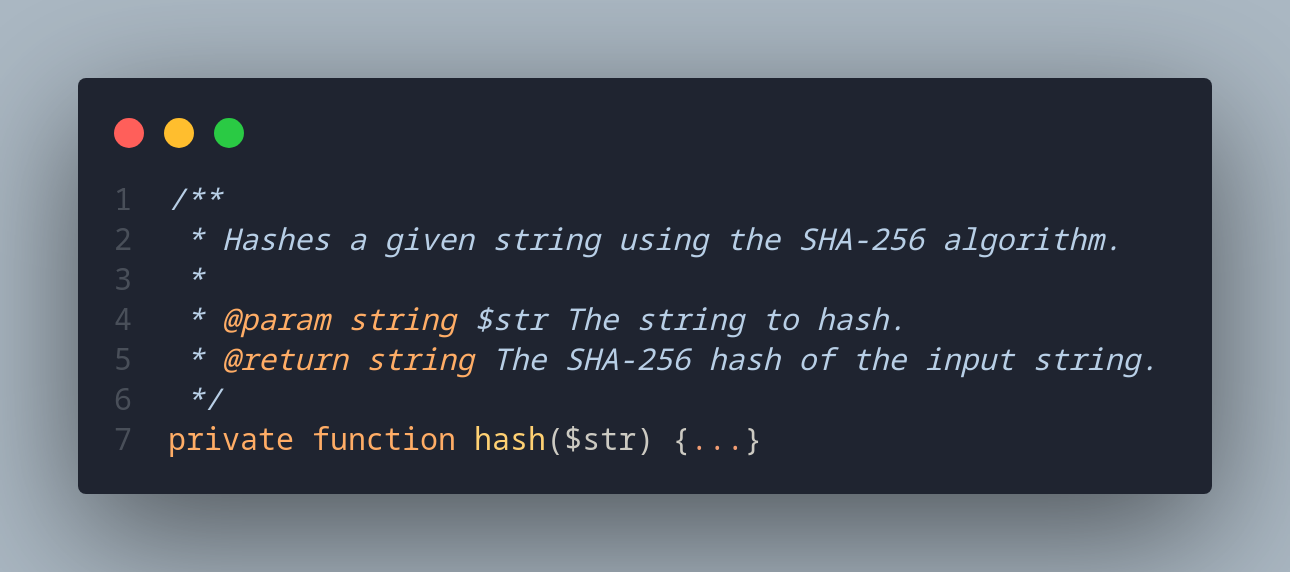
\includegraphics[page=1, width=1\textwidth]{hash.png}
\end{center}


\subsection{Testprotokoll}
\label{app:test}
\includegraphicsKeepAspectRatio{md/testprotokoll-1-1.png}{1}
\clearpage
\includegraphicsKeepAspectRatio{md/testprotokoll-2-1.png}{1}
\clearpage

\subsection{Klasse: ComparedNaturalModuleInformation}
\label{app:CNMI}
Kommentare und simple Getter/Setter werden nicht angezeigt.
\lstinputlisting[language=php, caption={Klasse: ComparedNaturalModuleInformation}]{Listings/cnmi.php}
\clearpage

\subsection{Klassendiagramm}
\label{app:Klassendiagramm}
Klassendiagramme und weitere \acs{UML}-Diagramme kann man auch direkt mit \LaTeX{} zeichnen, siehe \zB \url{http://metauml.sourceforge.net/old/class-diagram.html}.
\begin{figure}[htb]
\centering
\includegraphicsKeepAspectRatio{Klassendiagramm.pdf}{1}
\caption{Klassendiagramm}
\end{figure}
\clearpage

\subsection{Benutzerdokumentation}
\label{app:BenutzerDoku}

\justifying

\subsubsection{Starten des Programms}
Öffnen Sie den Webbrowser Ihrer Wahl und navigieren Sie zu \url{https://[domain]/einloesen}. Wenn Sie nicht eingeloggt sind, dann werden Sie nun zur Login-Seite weitergeleitet. Melden Sie sich hier mit Ihrem Mitgliedszugang von Contao an.

Nachdem Sie sich erfolgreich eingeloggt haben, werden Sie zur Startseite weitergeleitet.

Stellen Sie sicher, dass Ihre Kamera und Internetverbindung aktiviert sind, um alle Funktionen der Anwendung nutzen zu können.

\subsubsection{Scannen eines QR-Codes}
\textbf{QR-Code-Scanner öffnen:} Klicken sie auf der Startseite auf das QR-Code-Icon um den Scan-Prozess zu starten.

\textbf{Kamera ausrichten:} Richten Sie die Kamera Ihres Geräts auf den QR-Code des Tickets. Achten Sie darauf, dass der QR-Code vollständig im Sichtfeld der Kamera ist.

\textbf{QR-Code scannen:} Das Programm scannt den QR-Code automatisch und leitet Sie zur Ticketinformation weiter. Hier sehen Sie alle relevanten Details zur Bestellung.


\subsubsection{Entwertung des Tickets}

Nachdem der QR-Code erfolgreich gescannt wurde, können Sie das Ticket entwerten:

\textbf{Ticketinformationen überprüfen:} Stellen Sie sicher, dass die angezeigten Informationen mit den Daten des Gastes übereinstimmen.

\textbf{Ticket entwerten:} Klicken Sie auf die Schaltfläche "Ticket entwerten", um den QR-Code im System als eingelöst zu markieren.


\subsubsection{Fehlerbehebung beim Scannen}

Sollte der Scan fehlschlagen, gibt es einige Ansätze, um das Problem zu beheben:

\textbf{Lichtverhältnisse anpassen:} Starkes Sonnenlicht kann den Bildschirm eines Handys schwer erkennbar machen. Stellen Sie sich, wenn nötig, in den Schatten, um den QR-Code besser sichtbar zu machen.

\textbf{QR-Code vergrößern:} Wenn der QR-Code zu klein dargestellt wird, können Sie den Bildschirm vergrößern, um den QR-Code besser erkennbar zu machen. Nutzen Sie die Zoom-Funktion Ihres Geräts.


\subsubsection{Manuelle Suche für Tickets}

Falls der Scan-Prozess gerade nicht funktioniert, haben sie die Möglichkeit manuell nach Tickets zu suchen. Hierbei kann nach Datum, Bestellnummer oder Name gesucht werden.

\textbf{Zur Ticketliste wechseln:} Klicken Sie auf der Hauptseite oder im QR-Code-Scanner auf den Button mit der Lupe, um zur Ticketliste zu gelangen.

\textbf{Ticketnummer eingeben:} Geben Sie die Ticketnummer, Datum oder den Namen des Gastes in die Suchleiste ein.

\textbf{Ticket entwerten:} Wählen Sie das entsprechende Ticket aus der Liste aus und klicken Sie auf "Ticket entwerten", um es manuell zu entwerten.




\end{document}
